\newpage
\section{\label{ManipulatorModel}Manipulators}
\markright{\arabic{section}. Manipulators}
\hfill {\em documented by Hiromu Onda}


Instances of {\bf rotational-joint} class and {\bf manipulator} class 
constitute a Manipulator Model. {\bf rotational-joint} is a subclass of the 
{\bf body}. {\bf manipulator} is a subclass of the {\bf cascaded-coords}.
{\bf rotational-joint} class defines models of manipulator joints. 
{\bf manipulator} class has methods for solving a forward kinematic solution and 
inverse kinematic solution. 

The way of the definition of a manipulator is that i) Make all the 
joints of the manipulator, ii) Integrate these joints into {\bf manipulator}.



\subsection{
Rotational Joint
%\label{JointModel}Rotational Joint
}

{\bf rotational-joint} describes a model of a joint. 
{\bf rotational-joint} has {\bf body} as super-class.
This class manages a model of shape, coordinates, rotation axis of a joint, 
angles of rotation, limits of joint angles, etc.
{\bf defjoint} macro below creates an instance of {\bf rotational-joint}.
This instance is bound to {\em joint-name}. Assign a ancestor joint to 
{\bf parent}. It is not necessary to assign rotational axes to base nor 
fingers. 

\ptext{
(defjoint \= {\it joint-name} \hspace{0.5cm} \=  \\ % \hspace{4cm} \=\\
\>        :shape \> {\it body-object} \\
\>        :color \> {\it color-id} \hspace{2cm} \= ;0-15 for MMD \\
\>        :parent \> {\it parent-joint} \\
\>        :axis \> {\it rotational-axis} \>  ; :x, :y or :z \\
\>        :offset \> {\it trans-from-parent-joint} \\
\>        :low-limit \> {\it joint-angle-limit-low} \\
\>	  :high-limit \> {\it joint-angle-limit-hight} \\
\>        ) \\}

\subsection{
Multi-Joint Manipulators
%\label{MultiJointsManipulator}Multi-Joint Manipulators
}

A model of a manipulator is described by {\bf manipulator}. 
{\bf defmanipulator} macro below creates an instance of {\bf manipulator}. 

\ptext{
(defmanipulator {\it manipulator-name} \\
\hspace{2cm} \= :class \hspace{2cm} \= {\it manipulator-class} \\
\> :base \> {\it base-joint} \\
\> :joints \>  {\it list-of-all-joints} \\
\> :hand \> {\it handjoint} \\
\> :left-finger \> {\it left-finger}\\
\> :right-finger \> {\it right-finger}\\
\> :handcoords \> {\it trans-from-hand-to-armsolcoords}\\
\> :toolcoords \> {\it trans-from-armsolcoords-to-toolcoords} \\
\> :open-direction \> {\it finger-open-direction}\\
\> :right-handed  \> {\it righty-or-lefty} \\
\>        ) \\
}
\begin{refdesc}	
\classdesc{rotational-joint}{body}{(axis offset high-limit low-limit)}{
describes each rotational joint of a 6 D.O.Fs manipulator.}
\classdesc{manipulator}{cascaded-coords}{(\= base baseinverse joint\\
\> angles right-handed hand handcoords right-finger left-finger\\
\>openvec max-span toolcoords toolinverse armsolcoords\\
\> toolinverse armsocoords approach grasp affix)}
{manages kinematics of a manipulator from base to hand.}
\methoddesc{:newcoords} {newrot \&optional newpos}{ 
updates the coords with newrot and newpos if new joint angles are within the 
limit.
}
 \methoddesc{:armsolcoords } {}{
computes and makes transformation (an instance coords) 
between the coords of the 
base and those of the hand. 
}
 \methoddesc{:tool} {\&rest msg}{
modifies or gets toolcoords.
}
 \methoddesc{:set-tool} {newtool \&optional offset copy}{
sets new toolcoords.
}
 \methoddesc{:reset-tool } {}{
forces this coords to be default-toolcoords.
}
 \methoddesc{:worldcoords } {}{
computes the position vector, the rotation matrix, and the coordinates of the 
toolcoords represented in the world coordinates. 
}
 \methoddesc{:set-coords } {}{
forces setting coords according to the forward kinematic solution.
}
 \methoddesc{:config } {\&optional (a newangles)}{
sets joint angles of the manipulator.
}
 \methoddesc{:park } {}{
forces all the joint angles to be zero.
% 初期姿勢に戻す
}
\methoddesc{:hand}{\&optional (h nil)}{
sets or returns the object of its hand.
%  ハンドオブジェクトを返す
}
\methoddesc{:handcoords}{}{
computes the position vector, the rotation matrix, and the coordinates of the 
handcoords represented in the world coordinates. 
% ハンド座標系ののワールド表現を求める
}
\methoddesc{:span}{}{
returns the current distance between fingers.
%  現在の指の間隔を返す
}
\methoddesc{:open-fingers}{s \&optional abs \&aux (current (send self :span))}
{moves fingers relatively or absolutely.
% 指幅を相対的、絶対的に指定する
}
\methoddesc{:close-fingers} {}{
closes fingers completely.
% 指を完全に閉じる 
}
\methoddesc{:angles} {\&optional flag}{
returns the list of current joint angles.
% 現在の姿勢の関節角度のリストを返す
}
% \methoddesc{:right-handed} {}{
%% ソースそのものがありませんでした。
% 右手姿勢、左手姿勢を選択する
%}
 \methoddesc{:get-approach } {}{
returns the object to which the hand is approaching.
% 現在アプローチしている対象を返す
}
 \methoddesc{:set-approach } {a}{
sets {\it a} as the object to which the hand will approach.
% アプローチ対象を設定する
}
 \methoddesc{:get-grasp} {}{
(:get-grasp () grasp-config)
%??? 
% 把握姿勢にある対象物を返す
}
 \methoddesc{:set-grasp} {g}{
sets {\it g} as the object which the hand will grasp.
% 把握対象物を指定する
}
 \methoddesc{:get-affix} {}{
returns the object which the hand grasps.
% 把握している物体を返す
}
 \methoddesc{:affix} {\&optional (grasp)}{
sets {\bf affixed-object} {\bf grasp}.
{\bf grasp} is associated to the handcoords as a descendant. 
% 把握を指示する
}
 \methoddesc{:unfix} {\&optional (margin 10.0)}{
sets {\bf affixed-object} nil.
{\bf grasp} is dissociated (removed) from the descendants list of the handcoords.
% 把握物体を解放したことを指示する
}
\longdescription{:create}{\=\&rest args \`[method]\\
           \>\&key \=((:name nm)) ((:hand h)) ((:joints j))
                ((:left-finger lf)) ((:right-finger rf))\\
               \>\> ((:toolcoords tc) (make-coords))
                ((:handcoords hc) (make-coords))\\
                \>\>((:base bs) (make-cascoords))
                (open-direction (floatvector 0 1 0))\\
                \>\>((:max-span mspan) 100.0)
                ((:lefty lft) t)
                ((:act a) nil)\\
            \>\&allow-other-keys}{
creates and initializes a new manipulator object.
% 新しいマニピュレータオブジェクトを作成、初期化する
}

\end{refdesc}
{\bf manipulator} manages the linkage of the coords of 
{\bf base, joints(J1\ldots J6), handcoords, toolcoords}. 
{\bf manipulator} has {\bf cascaded-coords} as super-class. 
{\bf manipulator} is connected with {\bf base} which is {\bf cascaded-coords}
(or subclasses of {\bf body}). {\bf manipulator} manages the transformation from 
the base frame to the toolcoords. Messages sent to {\bf manipulator} 
(i.e. {\bf :translate, :locate, :rotate, :orient, :transform} etc.) effect 
the end effector of the manipulator. If WRT parameter is set one of keywords 
(i.e. :local, :parent, :world or an instance of coordinates) in this message, 
the end-effector  moves with respect to the WRT parameter. 
In the next program {\bf eta3} is a instance of {\bf manipulator}.

%{\bf manipulator}オブジェクトは、
%{\bf base、joints(J1\ldots J6)、handcoords、toolcoords}
%の座標系の連鎖を管理する。
%図\ref{ManipulatorObject}に{\bf manipulator}オブジェクトのスロット構成を、
%表\ref{ManipulatorMethods}に受け付けられるメソッドを掲げる。
%{\bf manipulator}クラスは、{\bf cascaded-coords}のサブクラスであり、
%やはり、{\bf cascaded-coords}(または{\bf body}などのサブクラス)
%である{\bf base}に結合され、
%{\bf base}から{\bf toolcoords}(手先座標系)への変換を管理している。
%したがって、{\bf manipulator}オブジェクトに対して送られる
%{\bf :translate、:locate、:rotate、:orient、:transform}
%などのメッセージは、手先点に対して作用する。
%そのとき同時にWRTパラメータを指定すれば、
%手先はWRT座標系に対して動く。
%次のプログラムでは、{\bf eta3}を{\bf manipulator}のインスタンスと仮定している。


\begin{verbatim}
 (send eta3 :translate #f(0 0 -100))        ;put back the end-effector by 10cm
 (send eta3 :translate #f(0 0 -100) :world) ;move down the end-effector by 10cm
 (send eta3 :translate #f(0 0 -100)
             (manipulator-base eta3))  ;move down the end-effector with respect 
                                       ;to the coords of the base by 10cm
\end{verbatim}

%\begin{verbatim}
% (send eta3 :translate #f(0 0 -100))        ;手先を10cm引っ込める 
% (send eta3 :translate #f(0 0 -100) :world) ;10cm下げる
% (send eta3 :translate #f(0 0 -100)
%             (manipulator-base eta3))     ;手先をベース座標系で10cm下げる
%\end{verbatim}

When {\bf manipulator} receives these messages, it calculates the arm solution 
and 6 joint angles are determined. Generally, more solutions than one exist.
In that case, one appropriate solution is chosen of them according to the 
criteria (i.e. the distinction between {\bf right-handed} and {\bf left-handed},
and the consistency with current joint angles). If there is no solution for 
a given configuration or the calculated joint angles exceed its limits, 
{\bf manipulator} does not move and it gives a warning.

%これらのメッセージに対して、manipulatorはアーム解を計算して6つの
%関節角度を決定する。
%一般に解は複数存在するが、{\bf right-handed}(右手系、左手系)
%の区別、および現在の関節角度との連続性により適当な解が選択される。
%しかし、指定された位置、姿勢に対する解が存在しない場合や関節角が
%限界を越える場合は移動、回転は起こらず、警告が発せられる。

Arm-solution method {\bf :armsol} must be defined for respective manipulator 
classes which correspond to real manipulators. This method calculates the 
transformation between the base-coords and the hand-coords. Thus this allow us 
to put a manipulator wherever with respect to the world-coords. The arm solution 
is independent of the {\bf base, toolcoords}.

%アーム解の計算は、実際のマニピュレータに対応した
%個々のmanipulatorクラスに定義された{\bf :armsol}メソッドが行う。
%マニピュレータがワールド座標系のどこに置かれてもよいように、
%また、どのような工具を用いてもよいように、アーム解は、
%{\bf base、toolcoords}とは独立に、base座標系中でのハンドの位置、姿勢に
%対して与えられる。

Fig. \ref{JointCoords} shows the relation between coordinate systems 
({\bf base, J1, J2,\ldots , handcoords} and {\bf toolcoords}). $T$ and other 
transformations are calculated as follows.

%{\bf base、J1、J2、\ldots 、handcoords、toolcoords}の関係を図\ref{JointCoords}
%に示す。
%ワールドから手先への変換を$T$とすると、$T$および各部分変換は次のようにし
%て得られる。

$
\begin{array}{ll}
T & = base \cdot J1 \cdot J2 \cdot \ldots 
\cdot J6 \cdot handcoords \cdot toolcoords \\ 
 & = (send \; eta3 \; :worldcoords) \\ 
T_{Jn} & = base \cdot J1\cdot \ldots \cdot Jn \\
 & = (send \; Jn \; :worldcoords) \\
T_{arm} & = J1 \cdot J2 \cdot \ldots \cdot J6 \cdot handcoords \\ 
 & = (send \; eta3 \; :armsol-coords) \\ 
T_{tool} & = J1 \cdot J2 \cdot  \ldots \cdot J6 \cdot handcoords \cdot toolcoords \\ 
 & = (send \; eta3 \; :copy-coords) \\
T_{t} & = toolcoords \\ 
 & = (manipulator-toolcoords \; eta3)\\
T_{t}^{-1} & = toolcoords^{-1} \\ 
 & = (manipulator-toolinverse \; eta3) \\
T_{h} & = handcoords \\ 
 & = (manipulator-handcoords \; eta3)\\
\end{array}$

where $T$ is the transformation between the world-coords and the toolcoords.

\begin{figure}
\begin{center}
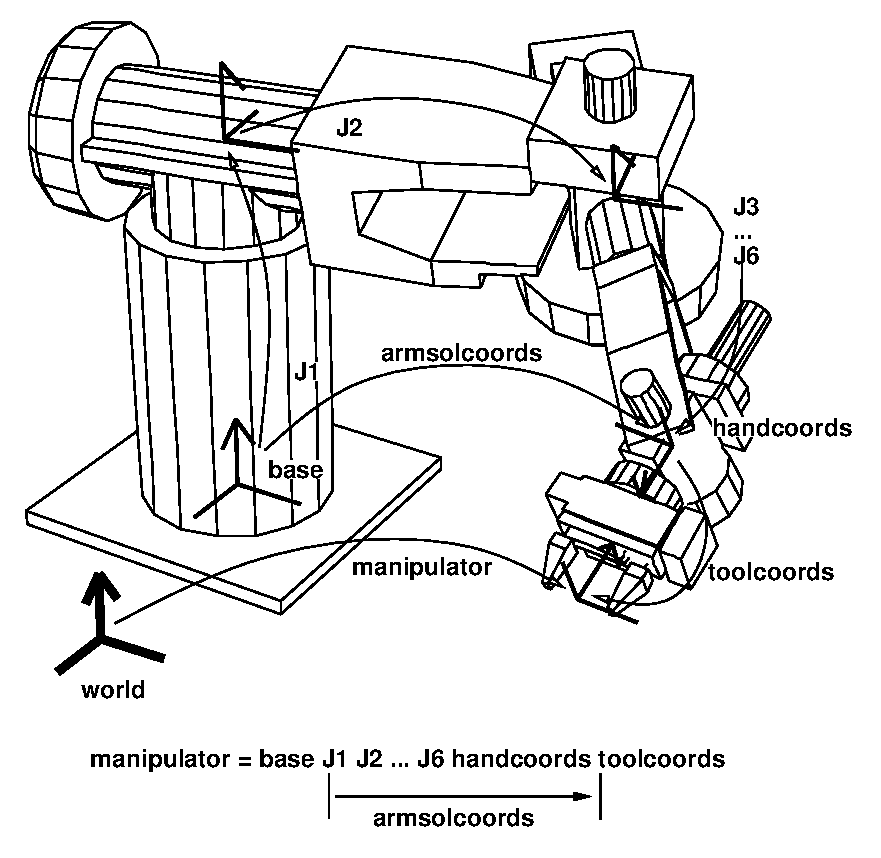
\includegraphics[height=100mm]{fig/eta3coords.ps}
%\epsfile{file=fig/eta3coords.ps,height=100mm}
%\mbox{
%\epsfysize=10cm
%\epsfbox{fig/eta3coords.ps}
%}
\end{center}
\caption{\label{JointCoords}
relation between coordinate systems in a manipulator}

\end{figure}

Each joint has a geometric model represented by Breps (Boundary Representation).
The coordinates of the vertices and the equations of the planes are not always 
current ones. Messages sent to {\bf manipulator} for translation or rotation only
update the coordinate systems, these do not update the coordinates of the 
vertices. This is why we can reduce the calculation time when translation or 
rotation occurs successively. If {\bf :worldcoords} message is sent to 
{\bf manipulator}, it updates the data such as the coordinates of the vertices.

%各関節は、Brepで表現された幾何モデルを保持している。しかし、頂点の座標、
%平面の方程式は常に現状を反映しているとは限らない。マニピュレータに対する
%移動、回転などのメッセージでは座標系の更新だけを行い、頂点の座標は変化し
%ない。これは、移動、回転が複数回続けて起こった場合の計算量を減らすためで
%ある。更新は、マニピュレータに{\bf :worldcoords}メッセージを送る
%ことで引き起こされる。

Mainly toolcoords are used for specify the motion of a manipulator in 
this {\bf manipulator}. There is a method ({\bf :config}) for specifying the 
configuration of the manipulator by joint angles. The arguments are a 
float-vector whose elements are 6.

%マニピュレータは、手先座標系で動作を指定することを主な目的としている。
%関節角による指定には {\bf :config} を用いる。
%引き数には6要素の列を与える。

\begin{verbatim}
  (send eta3 :config (float-vector pi/2 pi/2 0 1 0 1))
\end{verbatim}

{\bf :config} rotates joints of the manipulator if the joint angles are in the 
limit. As a result, the coordinates which {\bf manipulator} manages and the 
current toolcoords which given joint angles determines become inconsistent.
{\bf :set-coords} message must be sent if you need consistency. {\bf :set-coords}
calculates a forward kinematic solution and calculates the arm solution using the 
forward kinematic solution.


%{\bf :config}は、各関節角度が可動範囲に収まっていることを検査した後、
%それらを回転させる。
%この結果、マニピュレータの管理している座標系と
%関節角度から定まる実際の手先の位置姿勢とが一致しなくなる。
%両者を一致させるためには、{\bf :set-coords}メッセージを送る。
%{\bf :set-coords}は、関節角度から順方向のキネマティクスを計算し、
%最終的な手先座標系に対してさらにアーム解を解く。

Example: create the manipulator model (ETA3) and draw this on a Xwindow system.
\begin{verbatim}
;EusLisp 7.27 with Xlib created on Thu Sep 17 14:33:30 1992
(load "view.l")                                ;open a window
(load "/usr/local/eus/robot/eta3/eta3build.l") ;create the model of ETA3
(send *viewing* :look #f(2000 2000 2000))      ;change the viewpoint
(send-all (eta3arm-components eta3) :color 1)  ;change the color of lines
(send eta3 :config (float-vector 0 (/ -Pi 4.0) Pi/2 0 (/ -Pi 4.0) 0 ))
					       ;set joint angles of ETA3
(send eta3 :set-coords)                        ;refer to the above explanation
(draw eta3)                                    ;draw ETA3
\end{verbatim}


%例 ETA3のモデル生成とその描画
%\begin{verbatim}
%EusLisp 7.27 with Xlib created on Thu Sep 17 14:33:30 1992
%(load "view.l")                                ;ウィンドウを開く
%(load "/usr/local/eus/robot/eta3/eta3build.l") ;ETA3のモデルを生成する
%(send *viewing* :look #f(2000 2000 2000))      ;視点を変える
%(send-all (eta3arm-components eta3) :color 1)  ;物体の線の色を黒に変える
%(send eta3 :config (float-vector 0 (/ -Pi 4.0) Pi/2 0 (/ -Pi 4.0) 0 ))
%					       ;ETA3を関節角度の指定で動かす
%(send eta3 :set-coords)                        ;上記参照
%(draw eta3)                                    ;ETA3を描画する
%\end{verbatim}

\clearpage
